\documentclass[a0,landscape]{a0poster}

% ----------------------------------
% Packages essentiels
% ----------------------------------
\usepackage[utf8]{inputenc}
\usepackage[T1]{fontenc}
\usepackage{lmodern}
\usepackage{textcomp}
\usepackage{graphicx}
\usepackage{xcolor}
\usepackage{multicol}
\usepackage{geometry}
\usepackage{amsmath,amssymb}
\usepackage{float}
\usepackage{caption}
\usepackage{subcaption}
\usepackage{enumitem}
\usepackage{hyperref}
\usepackage{booktabs}
\usepackage{tikz}
\usepackage{tcolorbox}
\usepackage{fontawesome5}
\usepackage{array}


% ----------------------------------
% Configuration TikZ et tcolorbox
% ----------------------------------
\usetikzlibrary{shapes,arrows,positioning,shadows}
\tcbuselibrary{skins,breakable}

% ----------------------------------
% Mise en page générale
% ----------------------------------
\geometry{
  a0paper,
  landscape,
  top=1.5cm,
  bottom=1.5cm,
  left=1.5cm,
  right=1.5cm
}
\setlength{\columnsep}{1.5cm}
\setlength{\parindent}{0pt}

% ----------------------------------
% Couleurs personnalisées (palette moderne)
% ----------------------------------
\definecolor{primaryblue}{RGB}{41, 128, 185}
\definecolor{darkblue}{RGB}{52, 73, 94}
\definecolor{lightblue}{RGB}{174, 214, 241}
\definecolor{accentgreen}{RGB}{46, 204, 113}
\definecolor{accentorange}{RGB}{230, 126, 34}
\definecolor{accentred}{RGB}{231, 76, 60}
\definecolor{lightgray}{RGB}{245, 245, 245}
\definecolor{mediumgray}{RGB}{149, 165, 166}
\definecolor{textgray}{RGB}{44, 62, 80}

% ----------------------------------
% Styles personnalisés pour les boîtes
% ----------------------------------
\newtcolorbox{infobox}[1][]{
  colback=lightblue!20,
  colframe=primaryblue,
  arc=4mm,
  boxrule=2pt,
  left=8pt,
  right=8pt,
  top=8pt,
  bottom=8pt,
  #1
}

\newtcolorbox{resultbox}[1][]{
  colback=accentgreen!10,
  colframe=accentgreen,
  arc=4mm,
  boxrule=2pt,
  left=8pt,
  right=8pt,
  top=8pt,
  bottom=8pt,
  #1
}

\newtcolorbox{warningbox}[1][]{
  colback=accentorange!10,
  colframe=accentorange,
  arc=4mm,
  boxrule=2pt,
  left=8pt,
  right=8pt,
  top=8pt,
  bottom=8pt,
  #1
}

\newtcolorbox{criticalbox}[1][]{
  colback=accentred!10,
  colframe=accentred,
  arc=4mm,
  boxrule=2pt,
  left=8pt,
  right=8pt,
  top=8pt,
  bottom=8pt,
  #1
}

% ----------------------------------
% Styles pour les titres
% ----------------------------------
\usepackage{sectsty}
\allsectionsfont{\sffamily\bfseries\color{primaryblue}}

% Titre de section personnalisé
\newcommand{\bigsection}[1]{
  \vspace{0.5cm}
  \begin{tcolorbox}[
    colback=primaryblue,
    coltext=white,
    arc=2mm,
    boxrule=0pt,
    left=10pt,
    right=10pt,
    top=5pt,
    bottom=5pt
  ]
    {\Large\bfseries #1\par}
  \end{tcolorbox}
  \vspace{0.3cm}
}

% ----------------------------------
% Configuration des légendes
% ----------------------------------
\captionsetup{
  font={small,sf},
  labelfont={bf,color=primaryblue},
  labelsep=colon,
  justification=centering
}

% ----------------------------------
% Configuration des listes avec icônes
% ----------------------------------
\setlist{
  itemsep=0.3em,
  topsep=0.5em,
  partopsep=0pt,
  parsep=0.3em,
  leftmargin=1.2em
}

% Commandes pour des listes avec icônes
\newcommand{\checkitem}{\item[\textcolor{accentgreen}{\faCheck}]}
\newcommand{\infoitem}{\item[\textcolor{primaryblue}{\faInfoCircle}]}
\newcommand{\alertitem}{\item[\textcolor{accentorange}{\faExclamationTriangle}]}
\newcommand{\criticalitem}{\item[\textcolor{accentred}{\faTimes}]}

% ----------------------------------
% Commandes utiles
% ----------------------------------
\newcommand{\highlight}[1]{\textbf{\textcolor{primaryblue}{#1}}}
\newcommand{\metric}[2]{\textbf{\textcolor{accentgreen}{#1}}: #2}

% ----------------------------------------------------------------
% Document
% ----------------------------------------------------------------
\begin{document}

% ----------------------------------
% En-tête avec titre et logos
% ----------------------------------
\begin{tcolorbox}[
  colback=darkblue,
  coltext=white,
  arc=0mm,
  boxrule=0pt,
  left=20pt,
  right=20pt,
  top=15pt,
  bottom=15pt
]
\begin{center}
  {\Huge\sffamily\bfseries Classification de l'état de santé du fœtus}\\[0.3cm]
  {\LARGE\sffamily basée sur des données de Cardiotocographie}\\[0.8cm]
  {\Large\sffamily\textcolor{lightblue}{Timofey ABRAMOV \quad • \quad Yazan EL MAHMOUD \quad • \quad Selima KHESSAIRI}}\\[0.3cm]
  {\large\sffamily\textcolor{lightblue}{\faUniversity\ Projet SY09 — Printemps 2025}}
\end{center}
\end{tcolorbox}

\vspace{0.8cm}

% ----------------------------------
% Trois colonnes principales
% ----------------------------------
\begin{multicols}{3}
\raggedcolumns

%===========================
% Colonne 1
%===========================
\vspace{1em}
\bigsection{\faHeartbeat\ Contexte \& Problématique}
\vspace{1em}
\begin{infobox}
\textbf{\large Enjeu de santé publique}\\[0.3cm]
Selon l'ONU, près de \textbf{300 000 femmes} décèdent chaque année de complications liées à la grossesse. La cardiotocographie (CTG) permet de monitorer la santé fœtale, mais son interprétation reste complexe et subjective.
\end{infobox}

\vspace{0.5cm}

\begin{minipage}[t]{0.5\linewidth}  % Colonne gauche (50% de largeur)
\textbf{\color{primaryblue} Objectif de l'étude}
\begin{itemize}
  \checkitem Prédire efficacement la santé fœtale à partir de données CTG
  \checkitem Améliorer la détection précoce des situations à risque
  \checkitem Réduire la subjectivité de l'interprétation médicale
\end{itemize}

\begin{warningbox}
\textbf{\faExclamationTriangle\ Déséquilibre des classes}
\begin{itemize}[leftmargin=1em]
  \item Normal : \textbf{77,84\%} (1655 cas)
  \item Suspect : \textbf{13,87\%} (295 cas)  
  \item Pathologique : \textbf{8,27\%} (176 cas)
\end{itemize}
\end{warningbox}
\end{minipage}%
\hfill  % Espace flexible entre les minipages
\begin{minipage}[t]{0.45\linewidth}  % Colonne droite (45% pour éviter les débordements)
\begin{figure}[H]
  \centering
  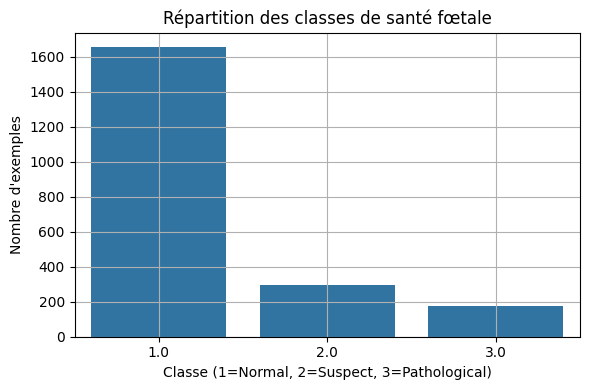
\includegraphics[width=\linewidth,height=10cm,keepaspectratio]{distribution_classes.png}
  \caption{Distribution de la variable cible (n=2126)}
  \label{fig:distrib_classes}
\end{figure}
\end{minipage}

\vspace{0.5cm}
\vspace{1em}
\bigsection{\faDatabase\ Jeu de Données}

\begin{infobox}
\textbf{Fetal Health Classification Dataset}\\
\faFile\ 2126 enregistrements CTG\\
\faList\ 21 variables descriptives numériques\\
\faCheckCircle\ Données complètes (pas de valeurs manquantes)\\
\faHospital\ Données cliniques réelles collectées en milieu hospitalier
\end{infobox}

\textbf{\color{primaryblue} Catégories de variables}
\begin{itemize}
  \infoitem \textbf{Rythme cardiaque fœtal} : valeur basale, variabilité, accélérations/décélérations
  \infoitem \textbf{Mesures utérines} : contractions, durée, valeur maximale
  \infoitem \textbf{Autres indicateurs} : mouvements fœtaux, activité anormale
\end{itemize}

\vspace{0.5cm}


\textbf{\color{primaryblue} Variables les plus corrélées à la cible}
\begin{itemize}
  \item \texttt{prolongued\_decelerations} (0.48)
  \item \texttt{abnormal\_short\_term\_variability} (0.47)  
  \item \texttt{percentage\_of\_time\_with\_abnormal\_long\_term\_variability} (0.43)
\end{itemize}

%===========================
% Colonne 2
%===========================
\vspace{1em}
\bigsection{\faSearch\ Analyse Exploratoire}
\vspace{1em}
\textbf{\color{primaryblue} Analyse en Composantes Principales}
\begin{itemize}
  \infoitem Les 2 premières composantes expliquent \textbf{45,55\%} de la variance
  \infoitem Séparation partielle des classes observée
  \infoitem Chevauchement important entre classes "suspect" et autres
\end{itemize}

\vspace{0.5cm}

\begin{figure}[H]
  \centering
  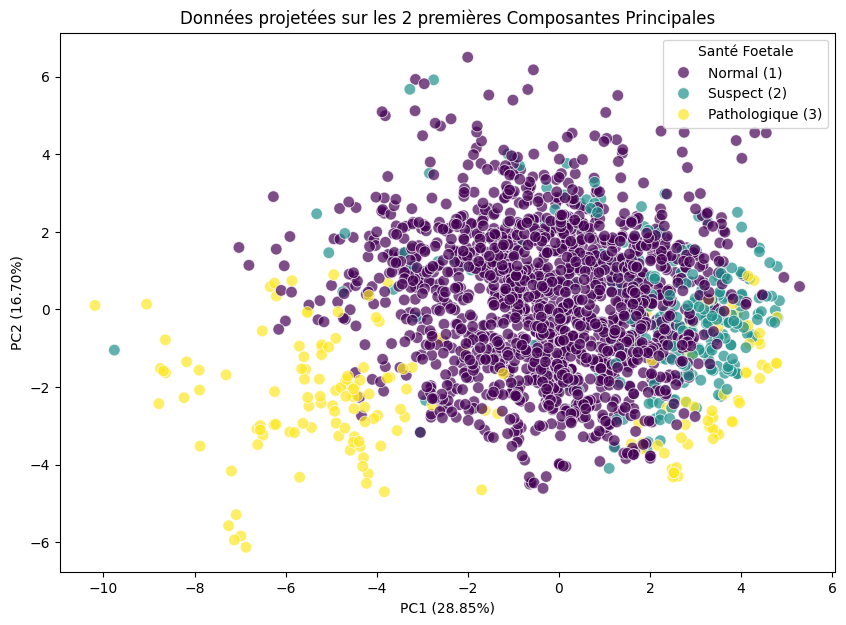
\includegraphics[width=0.9\linewidth,height=11cm,keepaspectratio]{acp_projection.png}
  \caption{Projection ACP - Premier plan factoriel}
  \label{fig:acp}
\end{figure}

\bigsection{\faCogs\ Approches Non Supervisées}

\begin{criticalbox}
\textbf{\faTimes\ Échec des méthodes non supervisées}
\begin{itemize}[leftmargin=1em]
  \item \textbf{K-means} : Indice de Rand ajusté très faible (0.045)
  \item \textbf{CAH} : Indice de Rand ajusté très faible (0.15)
  \item \textbf{Causes} : Chevauchement des classes, données non sphériques, haute dimensionnalité
\end{itemize}
\end{criticalbox}

\vspace{0.5cm}

\begin{figure}[H]
  \centering
  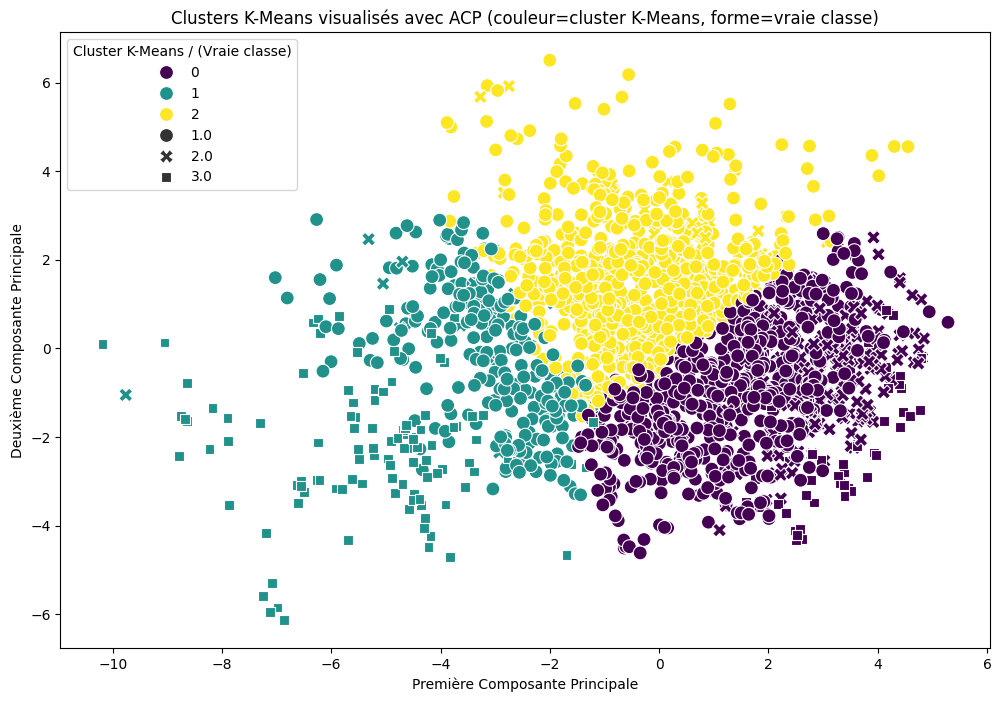
\includegraphics[width=0.85\linewidth,height=9cm,keepaspectratio]{kmeans_comparison.png}
  \caption{Comparaison K-means vs vraies classes}
  \label{fig:kmeans}
\end{figure}

\bigsection{\faRobot\ Approches Supervisées}

\textbf{\color{primaryblue} Stratégie d'évaluation}
\begin{itemize}
  \checkitem Données standardisées et stratifiées
  \checkitem Focus sur la détection des cas pathologiques
  \checkitem Prise en compte des coûts d'erreur asymétriques
\end{itemize}

\vspace{0.3cm}

\textbf{\color{primaryblue} Méthodes testées}
\begin{minipage}[t]{0.48\linewidth}
  \begin{itemize}
    \item K Plus Proches Voisins (k=4 optimal)
    \item Analyse Discriminante (LDA/QDA)
  \end{itemize}
\end{minipage}%
\hfill
\begin{minipage}[t]{0.48\linewidth}
  \begin{itemize}
    \item Naive Bayes Gaussien
    \item Régression Logistique
  \end{itemize}
\end{minipage}



%===========================
% Colonne 3
%===========================

\bigsection{\faChartLine\ Résultats des Modèles}

\begin{resultbox}
\textbf{\large Performances par algorithme}

\vspace{0.3cm}
\begin{tabular}{@{}l c c c@{}}
\toprule
\textbf{Modèle} & \textbf{Accuracy} & \textbf{Prec. Patho.} & \textbf{Rappel Patho.} \\
\midrule
\textcolor{accentgreen}{\textbf{Rég. Logistique}} & \textcolor{accentgreen}{\textbf{88,5\%}} & \textcolor{accentgreen}{\textbf{88\%}} & 66\% \\
KPPV (k=4) & 90,8\% & 84\% & 77\% \\
Arbres & 89,9\% & 81\% & 83\% \\
RF & 92\% & 87\% & 87\% \\
\bottomrule
\end{tabular}
\end{resultbox}

\begin{criticalbox}
\textbf{\large Performances par algorithme}

\vspace{0.3cm}
\begin{tabular}{@{}l c c c@{}}
\toprule
\textbf{Modèle} & \textbf{Accuracy} & \textbf{Prec. Patho.} & \textbf{Rappel Patho.} \\
\midrule
LDA & 85,9\% & 67\% & 46\% \\
QDA & 81,2\% & 76\% & 37\% \\
Naive Bayes & 81,0\% & 53\% & 46\% \\
\bottomrule
\end{tabular}
\end{criticalbox}

\vspace{0.5cm}

\textbf{\color{primaryblue} Analyse détaillée - Régression Logistique}

\begin{table}[H]
\centering
\small
\caption{Matrice de confusion - Régression Logistique}
\begin{tabular}{@{}l c c c@{}}
\toprule
\textbf{} & \textbf{Prédit Normal} & \textbf{Prédit Suspect} & \textbf{Prédit Pathologique} \\
\midrule
\textbf{Vrai Normal} & 314 & 17 & 1 \\
\textbf{Vrai Suspect} & 16 & 40 & 3 \\
\textbf{Vrai Pathologique} & 3 & 9 & 23 \\
\bottomrule
\end{tabular}
\end{table}

\begin{infobox}
\textbf{Points forts de la régression logistique multinomiale}
\begin{itemize}
  \checkitem Excellente reconnaissance des cas normaux (95\% rappel)
  \checkitem Précision remarquable sur les cas pathologiques (88\%)
  \alertitem Mauvaise reconnaissance des cas suspects
\end{itemize}
\end{infobox}

\bigsection{\faBalanceScale\ Approche Coût-Sensible}

\begin{table}[H]
\centering
\small
\caption{Matrice de coûts utilisée}
\begin{tabular}{@{}l c c c@{}}
\toprule
\textbf{} & \textbf{Prédit Normal} & \textbf{Prédit Suspect} & \textbf{Prédit Pathologique} \\
\midrule
\textbf{Vrai Normal} & 0 & 0.5 & 2 \\
\textbf{Vrai Suspect} & 1 & 0 & 1 \\
\textbf{Vrai Pathologique} & 5 & 4 & 0 \\
\bottomrule
\end{tabular}
\end{table}

\begin{warningbox}
\textbf{Stratégie médicale adaptée}\\
Privilégier les faux positifs plutôt que les faux négatifs critiques. Mieux vaut suspecter à tort une pathologie que de la manquer.
\end{warningbox}

\bigsection{\faLightbulb\ Conclusions \& Perspectives}

\textbf{\color{primaryblue} Contributions majeures}
\begin{itemize}
  \checkitem \textbf{Solution efficace} pour un problème médical complexe
  \checkitem Approche \textbf{interprétable} pour les praticiens
  \checkitem Méthodologie \textbf{adaptée aux enjeux cliniques} (coûts asymétriques)
  \checkitem Validation rigoureuse sur \textbf{données réelles}
\end{itemize}


\begin{warningbox}
\textbf{\faExclamationTriangle\ Limites actuelles}
\begin{itemize}[leftmargin=1em]
  \item Performance modérée sur les cas suspects
  \item Besoin de validation prospective
  \item Test de Wald non effectué
\end{itemize}
\end{warningbox}


\vspace{0.5cm}

\bigsection{\faBook\ Références}

\begin{enumerate}[label={[\arabic]},itemsep=0.15em,topsep=0.3em]
  \small
  \item ONU (2024). Statistiques sur la mortalité maternelle mondiale.
  
  \item Fetal Health Classification Dataset. UCI Machine Learning Repository.
  
  \item Pedregosa, F., et al. (2011). Scikit-learn: Machine Learning in Python. \emph{JMLR}, 12, 2825–2830.
\end{enumerate}

\end{multicols}

\end{document}